\documentclass[12pt]{article}
\usepackage{graphicx} % Required for inserting images
\usepackage{amsmath}
\usepackage{graphicx}
\usepackage{newtxtext,newtxmath} % Times New Roman font for text and math
\usepackage[a4paper, margin=1in]{geometry} % Adjust margins to resemble Word
\usepackage{caption} % For adding a caption without the figure environment
\usepackage{ragged2e} % For text justification
\title{DC Motor Control and Analysis}
\author{}
\date{}

\begin{document}

	\maketitle
	\vspace{-5em} % Adjust the value to decrease or increase the spacing
	
	\section*{Problem 1}
	The speed of a 10Hp, 210V, 1000 rpm separately excited DC motor is controlled by a single-phase full converter. The rated motor armature current is 30A and the armature resistance is 0.25 ohms. The AC supply voltage is 230V, and the motor voltage constant is 0.175 V/rpm. Assume continuous armature current for a firing angle of 45 degrees and rated armature current.
	
	Determine the following:	\begin{enumerate}
		\item The motor torque.
		\item The speed of the motor.
	\end{enumerate}
	
    \maketitle
    
    \noindent The average output voltage for a single-phase full converter is:
    \[
    V_{dc} = \frac{2V_m}{\pi} \cos \alpha
    \]
    where \( V_m = \sqrt{2} \times V_{rms} = \sqrt{2} \times 230 = 325.27\ \text{V} \). Substituting with \( \alpha = 45^\circ \):
    \[
    V_{dc} = \frac{2 \times 325.27}{\pi} \times \cos 45^\circ = 146.4\ \text{V}
    \]
    
    \noindent The back EMF \( E_b \) is:
    \[
    E_b = V_{dc} - I_a R_a = 146.4 - 30 \times 0.25 = 138.9\ \text{V}
    \]
    
    \noindent The motor speed \( N \) is:
    \[
    N = \frac{E_b}{K_e} = \frac{138.9}{0.172} = 807.6\ \text{rpm}
    \]
    
    \noindent The motor torque \( T \) is related to power by:
    \[
    P = T \times \omega, \quad \omega = \frac{2\pi N}{60}
    \]
    The power is:
    \[
    10\ \text{Hp} = 10 \times 745.7 = 7457\ \text{W}
    \]
    Now solve for torque:
    \[
    7457 = T \times \frac{2\pi \times 807.6}{60}
    \]
    \[
    T = \frac{7457}{\frac{2\pi \times 807.6}{60}} = 88.2\ \text{N}\cdot\text{m}
    \]


	
	\section*{Problem 2}
	A series DC motor is controlled by a single-phase half-controlled, full-wave rectifier bridge as shown in the figure. The AC input voltage has an RMS value of 240V at 50 Hz. The combined armature and field resistance is 2.5 ohms, and $K_{af} = 300\ \text{mH}$. If the load torque is 30 Nm and damping is neglected, calculate:
	\begin{enumerate}
		\item The average current.
		\item The speed for $\alpha = 60^\circ$.
	\end{enumerate}
	\begin{center}
		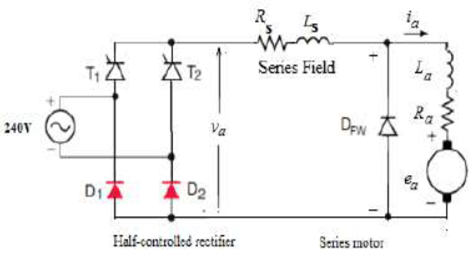
\includegraphics[scale=1.3]{pic1.png}
		\captionof{figure}{Motor Circuit}
	\end{center}
	
	\maketitle
	\noindent For a single-phase half-controlled rectifier, the average output voltage is given by:
	\[V_{dc} = \frac{V_m}{\pi} (1 + \cos \alpha)\]
	where \(V_m = \sqrt{2} \times V_{rms} = \sqrt{2} \times 240 = 339.4\ \text{V}\). Substituting the values:
	\[V_{dc} = \frac{339.4}{\pi} (1 + \cos 60^\circ) = 162.1\ \text{V}\]
	
	\noindent The motor equation for a series DC motor is:
	\[V_{dc} = I_a (R_a + R_f) + K_{af} \times \omega \times I_a\]
	Substituting \(V_{dc} = 162.1\ \text{V}\), \(I_a \times R = I_a \times 2.5\ \Omega\), and \(K_{af} = 0.3\ \text{H}\):
	\[162.1 = 10 \times 2.5 + 0.3 \times \omega \times 10\]
	Simplifying:
	\[162.1 = 25 + 3\omega\]
	\[\omega = \frac{162.1 - 25}{3} = 45.7\ \text{rad/s}\]
	
	\noindent The torque equation is:
	\[T = K_{af} \times I_a^2\]
	Substituting \(T = 30\ \text{Nm}\) and \(K_{af} = 0.3\ \text{H}\):
	\[30 = 0.3 \times I_a^2 \implies I_a = \sqrt{\frac{30}{0.3}} = 10\ \text{A}\]
	
	\noindent Finally, the motor speed in rpm is:
	\[N = \frac{\omega \times 60}{2\pi} = \frac{45.7 \times 60}{2\pi} = 436.4\ \text{rpm}\]
	

	\newpage
	
	\section*{Problem 3}
	The speed of a 10Hp, 220V, 1200 rpm separately excited DC motor is controlled by a single-phase fully controlled converter. The rated armature current is 40A, and the motor constant $K_\phi = 0.18\ \text{V/rpm}$. Assume that the motor current is constant and ripple-free for a firing angle of 30 degrees and rated motor current.
	
	Determine the following:
	\begin{enumerate}
		\item Speed of the motor.
		\item Motor torque.
		\item Power supplied to the motor.
	\end{enumerate}
	
	\maketitle
	
	\noindent The average output voltage for a single-phase fully controlled converter is:
	\[
	V_{dc} = \frac{2V_m}{\pi} \cos \alpha
	\]
	where \( V_m = \sqrt{2} \times 220 = 311.13\ \text{V} \). Substituting with \( \alpha = 30^\circ \):
	\[
	V_{dc} = \frac{2 \times 311.13}{\pi} \times \cos 30^\circ = 171.5\ \text{V}
	\]
	
	\noindent The back EMF \( E_b \) is given by:
	\[
	V_{dc} = E_b + I_a R_a
	\]
	Assuming \( E_b \approx V_{dc} \) for simplicity:
	\[
	E_b = 171.5\ \text{V}
	\]
	
	\noindent The motor speed \( N \) is:
	\[
	N = \frac{E_b}{K_\phi} = \frac{171.5}{0.18} = 952.8\ \text{rpm}
	\]
	
	\noindent The motor torque \( T \) is related to power by:
	\[
	T = \frac{P \times 746}{\frac{2\pi N}{60}}
	\]
	Substituting \( P = 10\ \text{Hp} \):
	\[
	T = \frac{10 \times 746}{\frac{2\pi \times 952.8}{60}} = 74.8\ \text{N}\cdot\text{m}
	\]
	
	\noindent The power supplied to the motor is:
	\[
	\text{Power supplied} = V_{dc} \times I_a = 171.5 \times 40 = 6860\ \text{W}
	\]
	
	
	\section*{Problem 4}
	The speed of a 10Hp, 220V, 1200 rpm separately excited DC motor is controlled by a single-phase fully controlled converter. The rated armature current is 40A, and the armature resistance is 0.25 ohms. The AC supply voltage is 230V. The motor constant $K_\phi = 0.18\ \text{V/rpm}$. Assume that the motor current is constant and ripple-free.
	
	For a firing angle of 30 degrees and rated motor current, determine the following:
	\begin{enumerate}
		\item Speed of the motor.
		\item Motor torque.
		\item Power supplied to the motor.
	\end{enumerate}
	
	\maketitle
	
	\noindent For a single-phase fully controlled converter, the average output voltage is given by:
	\[
	V_{dc} = \frac{2V_m}{\pi} \cos \alpha
	\]
	where \( V_m = \sqrt{2} \times V_{rms} = \sqrt{2} \times 230 = 325.27\ \text{V} \). Substituting the values with \( \alpha = 30^\circ \):
	\[
	V_{dc} = \frac{2 \times 325.27}{\pi} \times \cos 30^\circ = 180.1\ \text{V}
	\]
	
	\noindent The back EMF \( E_b \) is given by:
	\[
	E_b = V_{dc} - I_a R_a
	\]
	Substituting \( V_{dc} = 180.1\ \text{V} \), \( I_a = 40\ \text{A} \), and \( R_a = 0.25\ \Omega \):
	\[
	E_b = 180.1 - 40 \times 0.25 = 170.1\ \text{V}
	\]
	
	\noindent The motor speed \( N \) is given by:
	\[
	N = \frac{E_b}{K_\phi}
	\]
	where \( K_\phi = 0.18\ \text{V/rpm} \). Substituting:
	\[
	N = \frac{170.1}{0.18} = 945\ \text{rpm}
	\]
	
	\noindent The motor torque \( T \) is related to power by:
	\[
	P = T \times \omega
	\]
	where \( \omega = \frac{2\pi N}{60} \) is the angular velocity in radians per second. First, convert 10 Hp to watts:
	\[
	10\ \text{Hp} = 10 \times 745.7 = 7457\ \text{W}
	\]
	Now, calculate the torque:
	\[
	7457 = T \times \left( \frac{2\pi \times 945}{60} \right)
	\]
	\[
	T = \frac{7457}{\frac{2\pi \times 945}{60}} = 75.4\ \text{N}\cdot\text{m}
	\]
	
	\noindent Finally, the power supplied to the motor is:
	\[
	\text{Power supplied} = V_{dc} \times I_a = 180.1 \times 40 = 7204\ \text{W}
	\]
	
\end{document}
